%------------------------------------------------------------------------------
% Template file for the submission of papers to IUCr journals in LaTeX2e
% using the iucr document class
% Copyright 1999-2013 International Union of Crystallography
% Version 1.6 (28 March 2013)
%------------------------------------------------------------------------------


\documentclass[preprint]{iucr}              % DO NOT DELETE THIS LINE
\usepackage{amssymb}
\usepackage[fleqn]{amsmath}
%\usepackage{bm}
\usepackage{graphicx}
\usepackage{tabularx}
\usepackage{booktabs}
%\usepackage{calligra}
\usepackage{array}
\DeclareMathAlphabet{\mathcalligra}{T1}{calligra}{m}{n}
\def\mathbi#1{\textbf{\em #1}}
\numberwithin{equation}{section}
%\DeclareMathSymbol{\Gamma}{\mathalpha}{letters}{''00}
%\DeclareMathSymbol{\Lambda}{\mathalpha}{letters}{''03}
%\DeclareMathSymbol{\Omega}{\mathalpha}{letters}{''0A}
%\DeclareMathAlphabet{\mathitbf}{OML}{cmm}{b}{it}
\hyphenation{Niggli}
\def\mathbi#1{\textbf{\em #1}}
%\numberwithin{equation}{section}
%\DeclareMathSymbol{\Gamma}{\mathalpha}{letters}{''00}
%\DeclareMathSymbol{\Lambda}{\mathalpha}{letters}{''03}
%\DeclareMathSymbol{\Omega}{\mathalpha}{letters}{''0A}
%\DeclareMathAlphabet{\mathitbf}{OML}{cmm}{b}{it}
\usepackage{color}
\usepackage{ulem}
\usepackage{url}
\usepackage{yfonts}
%\usepackage{xr-hyper}
%\usepackage[draft]{hyperref}
%\usepackage{bibentry}
\newcommand{\SVI}[0]{$\bf{S^{6}}$}
\newcommand{\GVI}[0]{$\bf{G^{6}}$}
\newcommand{\CIII}[0]{$\bf{C^{3}}$}
\newcommand{\DVII}[0]{$\bf{D^{7}}$}
\newcommand{\VVII}[0]{$\bf{V^{7}}$}

\newcommand{\vdotv}[2]{${{\bf #1 \cdot #2}}$}
\newcommand{\Imaginary}[0]{\mathcal{I}}
\newcommand{\Real}[0]{\mathcal{R}}
\newcommand{\Exchange}[0]{$\mathcal{X}$}

\newcommand{\nounderline}[3]{\!\!\!\!\!\!\!\!\!#1,&\!\!\!\!\!\!\!\!\!#2,&\!\!\!\!\!\!\!\!\!#3}
\newcommand{\underlineab}[3]{\!\!\!\!\!\!\!\!\!\!\!\!\!\!\!\!\!\!\!\!\!\!\!\!\Exchange{}(#1),&\!\!\!\!\!\!\!\!\!\!\!\!\!\!\!\!\!\!\!\!\!\!\!\!\Exchange{}(#2),&\!\!\!\!\!\!\!\!\!#3}
\newcommand{\underlineac}[3]{\!\!\!\!\!\!\!\!\!\!\!\!\!\!\!\!\!\!\!\!\!\!\!\!\Exchange{}(#1),&\!\!\!\!\!\!\!\!\!\!\!\!\!\!\!\!\!\!\!\!\!\!\!\!#2,&\!\!\!\!\!\!\!\!\!\Exchange{}(#3)}
\newcommand{\underlinebc}[3]{\!\!\!\!\!\!\!\!\!\!\!\!\!\!\!\!\!\!\!\!\!\!\!\!#1,&\!\!\!\!\!\!\!\!\!\Exchange{}(#2),&\!\!\!\!\!\!\!\!\!\!\!\!\!\!\!\!\!\!\!\!\!\!\!\!\Exchange{}(#3)}

\newcommand{\scalar}[1]{$#1$}

\newcommand{\scalarsub}[2]{$#1_#2$}

%-------------------------------------------------------------------------
% Information about journal to which submitted
%-------------------------------------------------------------------------
\journalcode{J}              % Indicate the journal to which submitted
%   A - Acta Crystallographica Section A
%   B - Acta Crystallographica Section B
%   C - Acta Crystallographica Section C
%   D - Acta Crystallographica Section D
%   E - Acta Crystallographica Section E
%   F - Acta Crystallographica Section F
%   J - Journal of Applied Crystallography
%   M - IUCrJ
%   S - Journal of Synchrotron Radiation
\makeatletter
\font\dummyft@=dummy \relax
\makeatother


\begin{document}                  % DO NOT DELETE THIS LINE
	
	%-------------------------------------------------------------------------
	% The introductory (header) part of the paper
	%-------------------------------------------------------------------------
	
	% The title of the paper. Use \shorttitle to indicate an abbreviated title
	% for use in running heads (you will need to uncomment it).
	
	% Authors' names and addresses. Use \cauthor for the main (contact) author.
	% Use \author for all other authors. Use \aff for authors' affiliations.
	% Use lower-case letters in square brackets to link authors to their
	% affiliations; if there is only one affiliation address, remove the [a].
	
	% Use \vita if required to give biographical details (for authors of
	% invited review papers only). Uncomment it.
	
	% lca IUCr id IUCr6401
	%\vita{Author's biography}
	
	% Keywords (required for Journal of Synchrotron Radiation only)
	% Use the \keyword macro for each word or phrase, e.g. 
	% \keyword{X-ray diffraction}\keyword{muscle}
	
	
	% PDB and NDB reference codes for structures referenced in the article and
	% deposited with the Protein Data Bank and Nucleic Acids Database (Acta
	% Crystallographica Section D). Repeat for each separate structure e.g
	% \PDBref[dethiobiotin synthetase]{1byi} \NDBref[d(G$_4$CGC$_4$)]{ad0002}
	
	%\PDBref[optional name]{refcode}
	%\NDBref[optional name]{refcode}
	
	%-------------------------------------------------------------------------
	% The introductory (header) part of the paper
	%-------------------------------------------------------------------------
	
	% The title of the paper. Use \shorttitle to indicate an abbreviated title
	% for use in running heads (you will need to uncomment it).
	{\LARGE \emph{\today}} \\
	\title{A``Periodic Table'' for Bravais Lattices}
	%\title{Note on the transformation of three-space basis vectors to  corresponding matrix for Delaunay scalars}
	\shorttitle{A grid summarizing the Bravais lattice types according to Delaunay (Delone)}
	
	% Authors' names and addresses. Use \cauthor for the main (contact) author.
	% Use \author for all other authors. Use \aff for authors' affiliations.
	% Use lower-case letters in square brackets to link authors to their
	% affiliations; if there is only one affiliation address, remove the [a].
	
	
	\cauthor[a]{Lawrence C.}{Andrews}{larry6640995@gmail.com}{}
	\author[b]{Herbert J.}{Bernstein}
	
	\aff[a]{9515 NE 137th St, Kirkland, WA, 98034-1820 \country{USA}}
	\aff[b]{c/o NSLS-II, Brookhaven National Laboratory, Upton, NY, 11973 \country{USA}}
	
	% Use \shortauthor to indicate an abbreviated author list for use in
	% running heads (you will need to uncomment it).
	
	\shortauthor{Andrews and Bernstein}
	
	% Use \vita if required to give biographical details (for authors of
	% invited review papers only). Uncomment it.
	
	% lca IUCr id IUCr6401
	%\vita{Author's biography}
	
	% Keywords (required for Journal of Synchrotron Radiation only)
	% Use the \keyword macro for each word or phrase, e.g. 
	% \keyword{X-ray diffraction}\keyword{muscle}
	
	\keyword{lattice}
	\keyword{reduction}
	\keyword{Delone}
	\keyword{Selling}
	\keyword{Delaunay}
	
	% PDB and NDB reference codes for structures referenced in the article and
	% deposited with the Protein Data Bank and Nucleic Acids Database (Acta
	% Crystallographica Section D). Repeat for each separate structure e.g
	% \PDBref[dethiobiotin synthetase]{1byi} \NDBref[d(G$_4$CGC$_4$)]{ad0002}
	
	%\PDBref[optional name]{refcode}
	%\NDBref[optional name]{refcode}
	
	\maketitle                        % DO NOT DELETE THIS LINE
	
	\begin{synopsis}
		
		A tabular arrangement of the Bravais lattice types as
		defined by Delaunay is described.

	\end{synopsis}
	\newcommand{\si}[0]{$s_1$}
	\newcommand{\sii}[0]{$s_2$}
	\newcommand{\siii}[0]{$s_3$}
	\newcommand{\siv}[0]{$s_4$}
	\newcommand{\sv}[0]{$s_5$}
	\newcommand{\svi}[0]{$s_6$}
	\newcommand{\Svec} [0] {\{\si, \sii, \siii, \siv, \sv, \svi \}}
	\newcommand{\SvecA} [0] {\{-\si, -\si+\sii, \si+\siii, \si+\sv, \si+\siv, \si+\svi \}}
	
	\newcommand{\OPES}[0]{$E^3toS^6$}
	\newcommand{\OPESS}[0]{$$E^3toS^6$$}
	\newcommand{\MSVI}[0]{$M_{S^{6}}$}
	\newcommand{\MEIII}[0]{$M_{E^{3}}$}
	\newcommand{\Plus}[0]{\mathcal{P}}	
	\newcommand{\Minus}[0]{\mathcal{M}}
	
	\newcommand{\ci}[0]{$c_1$}
	\newcommand{\cii}[0]{$c_2$}
	\newcommand{\ciii}[0]{$c_3$}
	
	
	\begin{abstract}
		
		A convenient tabular display of the Bravais lattices types
		as defined by Delaunay (using Selling reduction) is described.

		
		{\bf Note:}  In his later publications, Boris Delaunay used the Russian version of his surname, Delone.\\
		
		
	\end{abstract}
	% Appendices appear after the main body of the text. They are prefixed by
	% a single \appendix declaration, and are then structured just like the
	% body text.
	
	\section{stuff for larry to do}
	supplementary material -- should there be a PDF file?/????
	
	
	\section{Introduction}
	\citeasnoun{kahr2023periodic} suggested a``Periodic table of the space groups''. In the
	same spirit, a ``Periodic Table'' of the Bravais lattice types is presented here.
	The table presents a systematic arrangement of the types, according to suggestions
	by \citeasnoun{Delaunay1932}. Like the periodic table of the elements, a brief amount
	of useful information is included.
	
\section{The space \SVI{}}
	
		The scalars used by~\citeasnoun{Delaunay1932} in his formulation of Selling reduction ~\cite{Selling1874}
	are (in the conventional order) $b \cdot c$, $a \cdot c$, $a \cdot b$, $a \cdot d$, 
	$b \cdot d$, $c \cdot d$, where $d = -a-b-c$. 
	(As a mnemonic device, 
	observe that the first three terms use
	$\alpha$, $\beta$, and $\gamma$, 
	in that order, 
	and the following terms use $a$, $b$, $c$, in that order.)
	
	~\citeasnoun{andrews2019b} chose to 
	represent the Selling scalars in the space \SVI{},
	\Svec{} (defined in the order above), 
	as a way to create a metric space
	for the measurement of the distance between lattices. 

		
	
\section{The table}

	\citeasnoun{Delaunay1932} and \citeasnoun{Delone1975} published a table of the Bravais types
	as distinguished by Selling (Delaunay) reduction.\cite{andrews2023measuring} published
	a somewhat modified version of Delaunay's table. The table presented here
	is arranged with the lattice family types as columns and the Federov polyhedron
	types as rows.
			\begin{figure}
		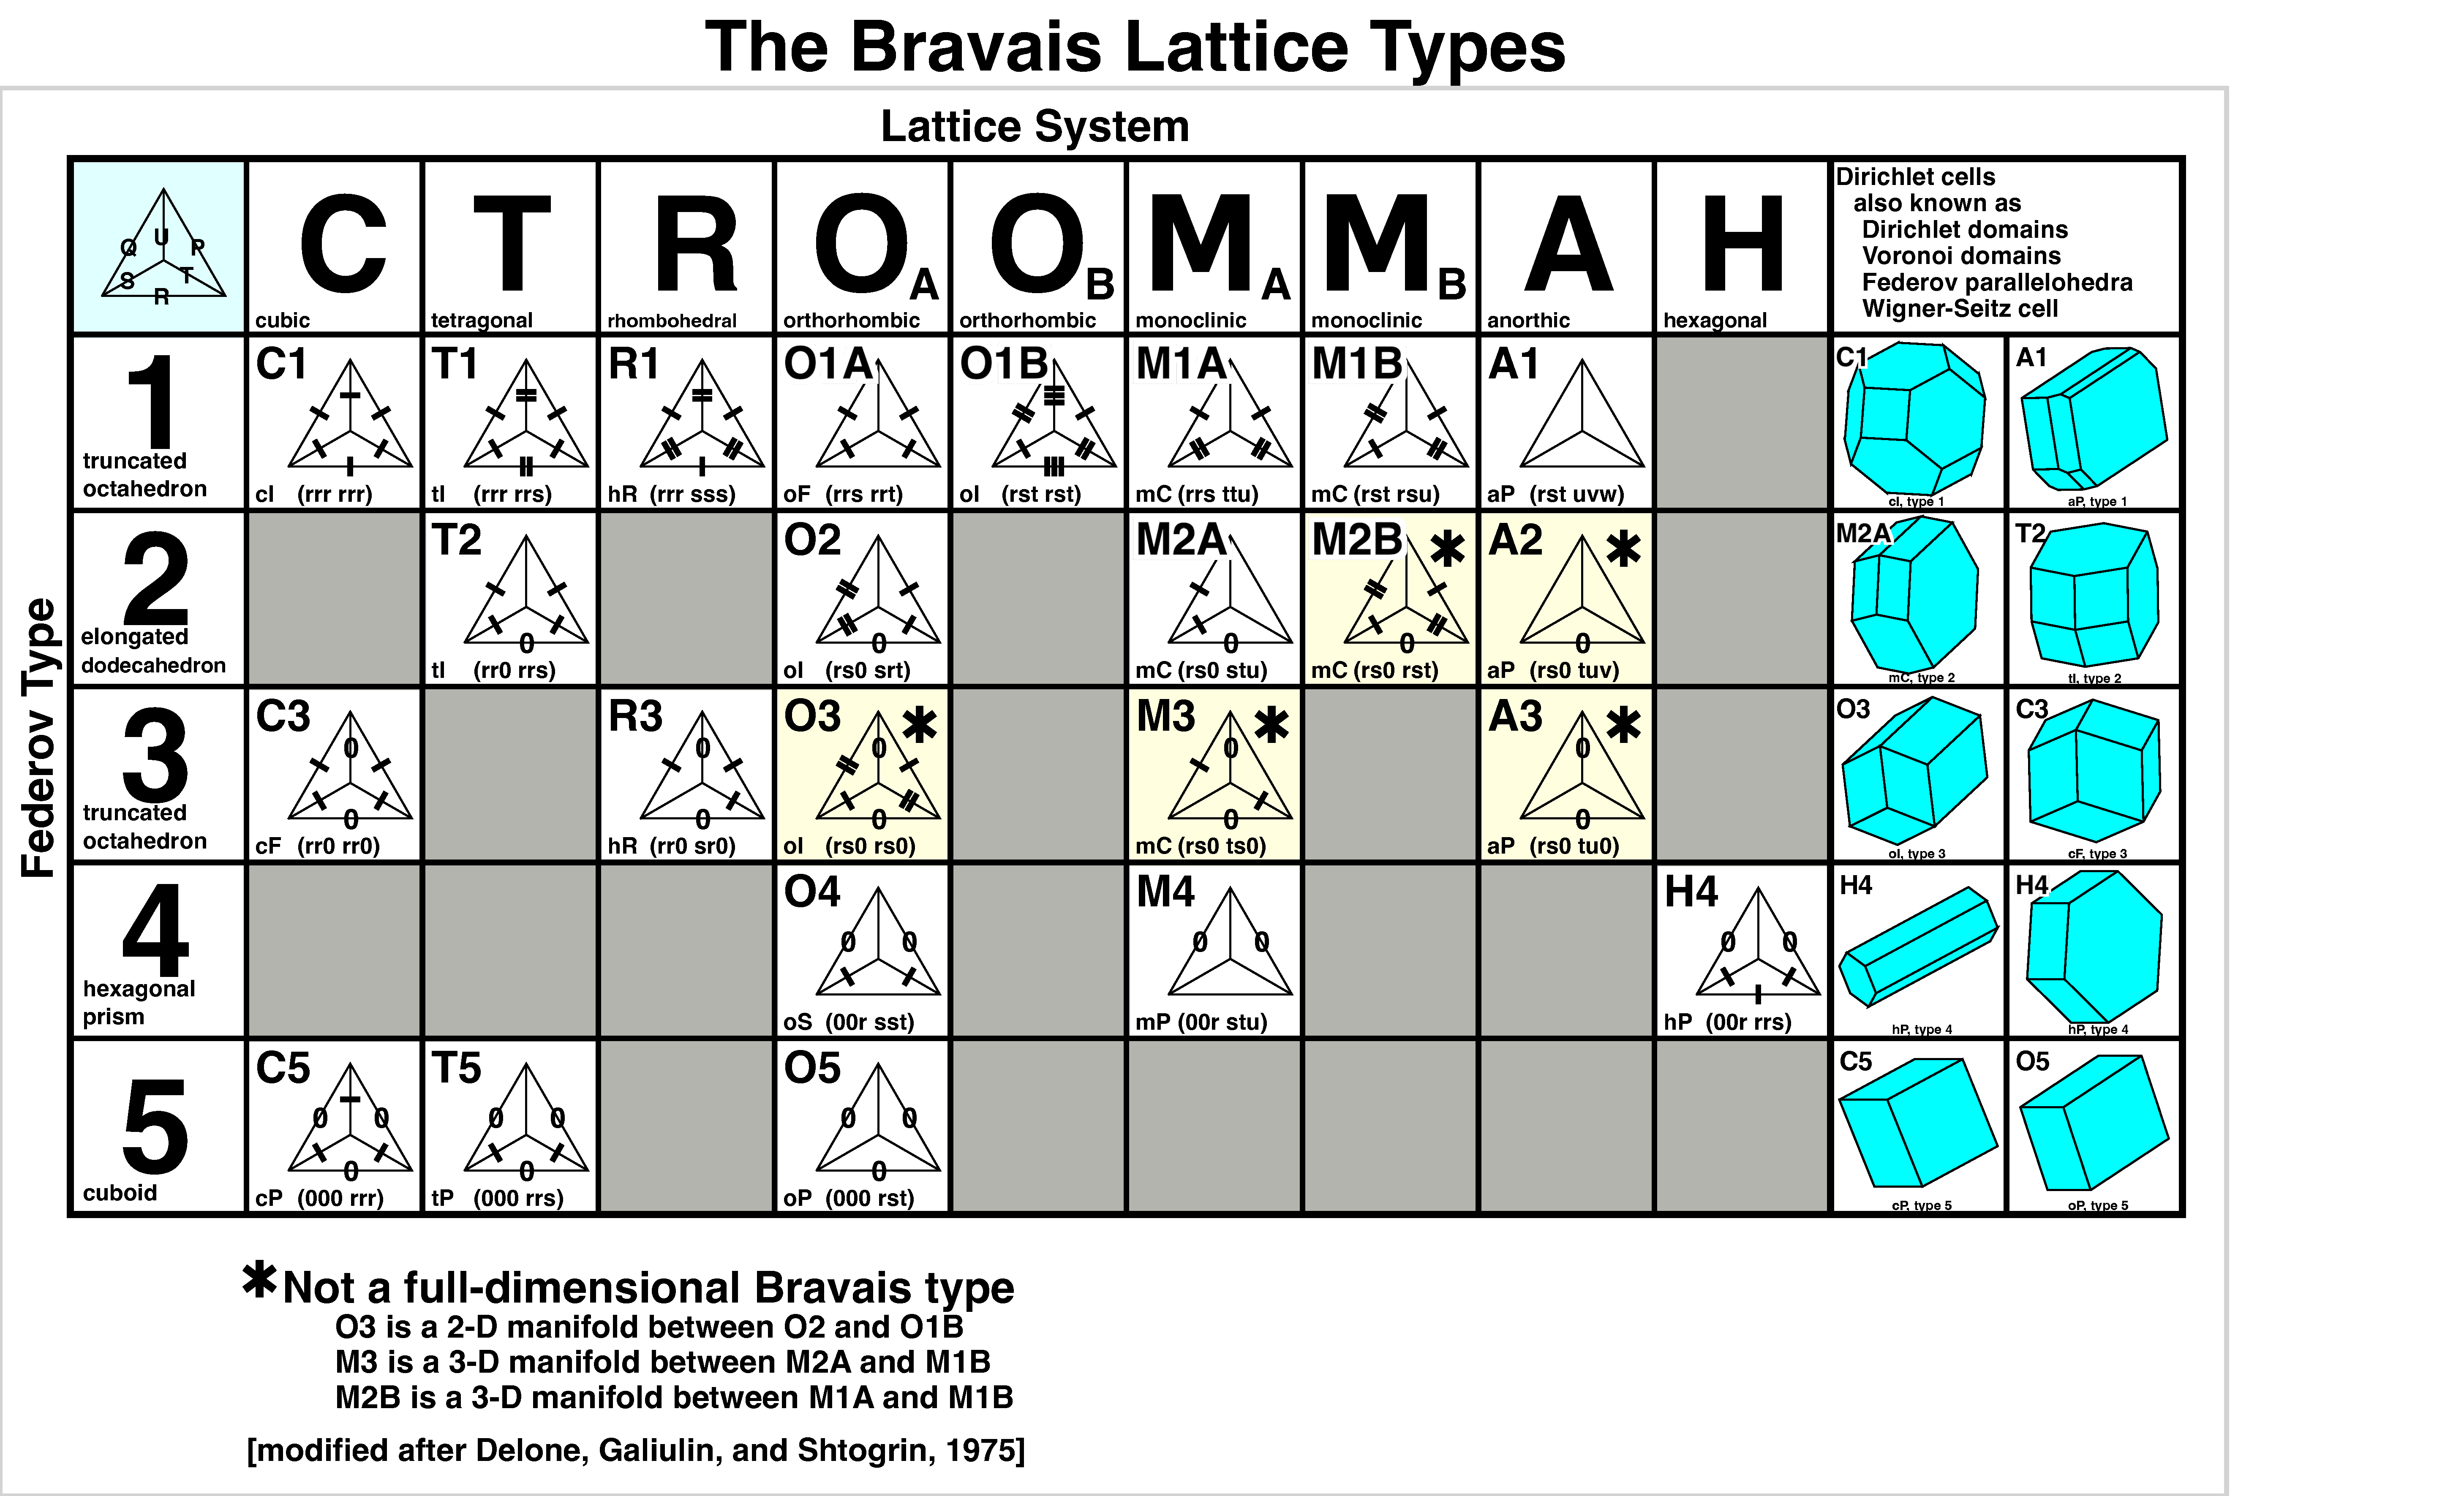
\includegraphics[width=10cm]{HorizontalDeloneGrid}
		\label{grid}
		\caption{The  Bravais lattice types.}
	\end{figure}
	
\section{The labeling of the columns (lattice families)}
	
	The columns are labeled according to the lattice family: cubic,
	tetragonal, rhombohedral, orthorhombic, monoclinic, and
	triclinic (anorthic). The labels for each reflect the names:
	\textbf{C}, \textbf{T}, \textbf{R}, \textbf{O},\textbf{ M}, \textbf{A}, \textbf{H} (rather than the choices of Delaunay: \textbf{K}, \textbf{Q},
	\textbf{R},\textbf{ O},\textbf{ M}, \textbf{T}, \textbf{H}, respectively).
	
	A further change from the model of Delaunay is the splitting 
	of orthorhombic and monoclinic into a pair of columns each
	($\bf{O_A}$, $\bf{O_B}$, $\bf{M_A}$, $\bf{M_B}$). This change 
	improved the display of these types. Delaunay had merged these
	disparate types into a single cell when their Federov
	types were identical. Thus, column $\bf{O}$ of \citeasnoun{Delaunay1932}
	has become columns $\bf{O_A}$ and $\bf{O_B}$, etc.
		
\section{The key cell (PQRSTU)}

The International Tables for x-ray crystallography \cite{vonLaue1952}
used the convention of labeling Selling parameters in the Bravais
tetrahedron, as \textbf{P}, \textbf{Q}, \textbf{R}, \textbf{S}, \textbf{T}, \textbf{U}, corresponding to the \SVI{} scalars
\Svec, respectively. For reference,
the figure has been included in the upper left cell of the table.
		\begin{figure}
		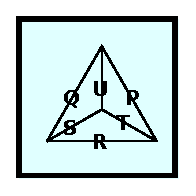
\includegraphics[width=5cm]{PQRSTU}
		\label{PQRSTU}
		\caption{The key cell with the labels used in the
		International Tables}
	\end{figure}
	
\section{The rows (Federov types)}
	
	\citeasnoun{fedorov1885elements} determined that there are only
	five kinds of parallelohedra that can be translated without rotations in 3-dimensional Euclidean space to fill space. 
	
	Except for rows 3 and 4, each row has a unique number of zero
	parameters. For rows 3 and 4, the difference is whether the two
	zeros are on opposite sides of the tetrahedron or on 
	adjacent sides.
	
\section{The cells}
	
		In the table described here, the conditions for each Delone
	type are described using \SVI{}. For example, the cell for
	primitive cubic lattices is $\bf{C5}$.
	
	
	\begin{figure}
		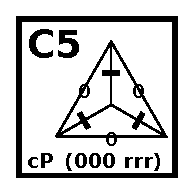
\includegraphics[width=5cm]{C5}
		\label{C5}
		\caption{The cell for the primitive cubic Bravais lattice type.}
	\end{figure}
	
	 $\bf{C5}$ is the label for the position (row and column, cubic and Federov type 5 reduced cell) within
	 the table. The stylized tetrahedron shows which Selling
	 parameters are zero or equal to each other. ``cP'' is the
	 standard display for primitive cubic.
	
	The \SVI{} characteristic for that type is (000 rrr); 
	
	\noindent
	\si{} = $b \cdot c$ = 0 ($\alpha$ = 90$^{\circ}$)\\
	\sii{} = $a \cdot c$ = 0 ($\beta$ = 90$^{\circ}$)\\
	\siii{} = $a \cdot b$ = 0 ($\gamma$ = 90$^{\circ}$)\\
	\siv{} = \sv{} = \svi{}	
	
\section{Dirichlet cells}

	At the right end of the table, a few examples of Dirichlet
	cells for each row. 
	
	
	\cite{fedorov1885elements}
	
	
\section{The unused/vacant cells}

	Prominent in the table are cells shown in gray. They have no
	corresponding Bravais type. For instance, the cell that would be
	$\bf{H1}$ would be a hexagonal cell with no zero parameters
	(this is no 90$^{\circ}$ angles); 
	clearly impossible. 
	
	
	
\section{Other changes from Delaunay}

	Within the table there are five cells that have a yellow
	background. Although Delaunay identified these among the 24
	Bravais types, they are special in the sense that they
	do no possess the full dimensionality of their lattice
	family. Most likely, they are only of minor crystallographic 
	interest.
	
	Cells $\bf{A1}$ and $\bf{A2}$ are triclinic unit cells with 
	one or two 90$^{\circ}$ angles. Respectively, they have only five
	or four free parameters.
	
	$\bf{O3}$ is a 2-D manifold that is the boundary between
	 $\bf{O2}$ and $\bf{O1B}$.
	With a characteristic of (rs0 rs0), $\bf{O3}$ has only two
	free parameters, not the three that is normal for an 
	orthorhombic unit cell.
	
	

%.\cite{andrews2023measuring}
%The table of Delaunay (1932) describing the 24 Bravais types in S6. It has
%been redone removing the images of the Dirichlet cells, the non-reduced
%cells, and adding the ‘lattice character’, which describes the linear
%manifold of each type. The crystal family types have been renamed to
%modern usage: Q changed to T for tetrahedral, K changed to C for cubic
%and T changed to A for anorthic. Where Delone in some places included
%two types in one table cell, they have been split into two (for example:
%‘M1’ is split into ‘M1A’ and ‘M1B)’. Note that five types (O3, M3, M2B,
%A2 and A3) are not normal crystallographic types. They are boundary
%types, and they have fewer free parameters than the generic type requires.
%For instance, O3 (character: rs0 rs0) has only two free parameters (r and
%s), whereas an ordinary orthorhombic type requires three variables.

%\begin{figure}
%	\includegraphics[width=1.0\textwidth]{7_14}
%	\label{7_14}
%		\caption{The same cells as plotted in Figure \ref{5_38} 
%	and Delone reduced, and then each multiplied by the 24
%	\SVI{} reflections.}
%\end{figure}
	
	\section{Summary}
	
\section{Supplementary Material}

The supplementary material includes the 
svg (Scalable Vector Graphics) file that generates the table.
	
	%\appendix
	
	
	
	\ack{{\bf Acknowledgements}}
	
	Careful copy-editing and corrections by Frances C. Bernstein are 
	gratefully acknowledged.

	\ack{{\bf Funding information}}      
	
%	Funding for this research was provided in part by:  
%	US Department of Energy Offices of Biological and 
%	Environmental Research and of Basic Energy Sciences 
%	(grant No. DE-AC02-98CH10886; grant No. E-SC0012704); 
%	U.S. National Institutes of Health (grant No. P41RR012408; 
%	grant No. P41GM103473; grant No. P41GM111244; 
%	grant No. R01GM117126,
%	grant No. 1R21GM129570); Dectris, Ltd.
	
	
	\bibliography{Reduced}
	
	\bibliographystyle{iucr}
	
	
	
	%-------------------------------------------------------------------------
	% TABLES AND FIGURES SHOULD BE INSERTED AFTER THE MAIN BODY OF THE TEXT
	%-------------------------------------------------------------------------
	
	% Simple tables should use the tabular environment according to this
	% model
	
	% Postscript figures can be included with multiple figure blocks
	
	%C:\Users\lca\Source\Repos\LatticeRepLib\x64\Debug>plotc3
	%; Graphical output SVG file =PLT__2023-03-07.13_43_35.svg
	%
	%C:\Users\lca\Source\Repos\LatticeRepLib\x64\Debug>cmdniggli | plotc3
	%; Graphical output SVG file =PLT__2023-03-07.13_44_06.svg
	%
	%C:\Users\lca\Source\Repos\LatticeRepLib\x64\Debug>cmddelone | plotc3
	%; Graphical output SVG file =PLT__2023-03-08.07_11_03.svg
	%
	%C:\Users\lca\Source\Repos\LatticeRepLib\x64\Debug>cmdniggli | cmdperturb 5 20 | plotc3
	%; Graphical output SVG file =PLT__2023-03-08.09_00_13.svg
	%
	%C:\Users\lca\Source\Repos\LatticeRepLib\x64\Debug>cmdniggli | cmdperturb 5 100 | plotc3
	%; Graphical output SVG file =PLT__2023-03-08.09_00_21.svg
	
\end{document}                    % DO NOT DELETE THIS LINE
%%%%%%%%%%%%%%%%%%%%%%%%%%%%%%%%%%%%%%%%%%%%%%%%%%%%%%%%%%%%%%%%%%%%%%%%%%%%%%
